\chapter{A general spectral collocation method for computing the dispersion relations of guided acoustic waves in multilayer dissipative structures}
\chaptermark{SCM for computing the dispersion relations of guided acoustic waves }
Authored by: \textit{Mathieu Maréchal, Alan Geslain, Jean-Philippe Groby and Vicent Romero-Garc\'ia}. 

\begin{center}
    {\color{gray}\textsc{This chapter is based on the material published in \cite{marechal2025}. Minor modifications to the text and figures have been made to fit the format and notation of this thesis.}}
\end{center}

\section{Abstract}
A spectral collocation method is proposed to compute the complex wavenumber-real frequency dispersion relations of guided acoustic waves in multilayer structures involving dissipative materials. The nature of these dissipative materials is initially considered to be arbitrary, i.e., poroelastic, viscoelastic, or viscoacoustic. For a given frequency, the complex wavenumbers as well as the physical fields, which are further used to evaluate the Poynting vectors and analyze the energy flux, are obtained by solving a generalized eigenvalue problem. The latter arises from a set of discretized equations of motion and appropriate boundary (coupling) conditions. These equations of motion and boundary (coupling) conditions are imposed by the nature of the material composing each layer of the structure. A focus is made on poroelastic layers. The dispersion relation of a two-layer elastic-poroelastic structure is analyzed, as well as the energy flows in the structure. The results as calculated with the present spectral collocation method are validated against those obtained with a classical complex root-finding (M\"uller) method and experiments.

%    \modif{Keywords: Spectral collocation method, poroelastic material, Complex dispersion relation, guided waves}
% \end{abstract}

% \maketitle

\section{Introduction}
Dealing with guided acoustic waves in multilayer stuctures of dissipative (viscoelastic, viscothermal, or poroelastic) material  requires the evaluation of complex wavenumber-real frequency dispersion relations. Solving for these dispersion relations consists in finding complex roots of complex characteristic equations, which often arise from complex matrix determinants and can rarely be solved analytically. Various methods \cite{ kowalczyk2017, dubbelday1983}, among which the Müller algorithm \cite{muller1956}, are commonly used to achieve this challenging task. These methods usually rely on preliminary semi-analytical derivations, require multiple initial guesses, and are iterative, so they can get stuck in local minima. Computing the complex wavenumber-real frequency dispersion relation in a reliable and robust way is thus of primary importance. Several numerical methods can be used, such as the Finite Element Method \cite{treyssede2014}, the Semi-Analytical Finite Element method (SAFE) \cite{bartoli2006, marzani2008,rose2014}, or spectral methods \cite{canuto2006}. Spectral methods are especially relevant in this framework. They are numerical approximation techniques that seek the solution of a differential equation using a finite series of infinitely differentiable basis functions with \emph{spectral accuracy} \cite{trefethen2000}.
    
The propagation and dispersion of waves in multilayer systems have long been investigated~\cite{lowe1995,haskell1953}. \modif{Citer \cite{huber2018, huber2023}, plutôt parler de TMM ou présenter logiciels existants (DISPERSE, dispersion box, GEWtool, etc.) ?} Spectral methods have been developed to cope with wave radiation problems, but have also emerged in the last decades to solve dispersion relations~\cite{pagneux2001}. Effectively, the numerical scheme boils down to discretizing the geometry along the layer thickness and solving an eigenvalue problem. Here, a collocation method is used to discretize the geometry. A finite-dimension polynomial basis is chosen and the collocation points are distributed according to the roots of this polynomial basis. Leaky modes appear in practice when multilayer structures are surrounded by one or two half-spaces. Accounting for this phenomenon brings us closer to practical considerations regarding these systems, as they would radiate part of the acoustic energy back to the surrounding medium, although it adds hardships to the modeling of the system; the waves modeled in these half-spaces should satisfy some radiation condition. These can be imposed by implementing perfectly matched layers \cite{gallezot2017}, by using a bounded mapping, and applying a Spectral Collocation Method (SCM) to all layers of the extended system \cite{georgiades2022}, or by using a suitable change of variable and solving a non-linear eigenvalue problem \cite{kiefer2019}. This last method inspires the current work. We propose a SCM suitable for solving complex wavenumber-real frequency dispersion relations in multilayer systems involving dissipative media. As a way of example, we will focus on multilayer poroelastic systems. Mechanical wave propagation in bulk poroelastic materials are well understood and modeled thanks to the seminal contributions of M.A. Biot \cite{biot1956,biot1956a,biot1962,biot1962a} and subsequent contributions, notably by D.L. Johnson \etal \cite{johnson1987} and J.-F. Allard \etal \cite{champoux1991,lafarge1997} concerning the modeling of viscothermal losses. Although poroelastic materials are bounded in practice and are usually encapsulated in more complex multilayer structures combining layers of materials of different nature in geophysics and acoustics, there are only a few studies on the dispersion relation of guided acoustic waves in poroelastic \cite{weisser2016, boeckx2005, belloncle2003}, porous \cite{allard2004,groby2008a} or anisotropic poroelastic layers \cite{seyfaddini2021}. The SCM has already been used to solve the dispersion relation of guided acoustic waves in elastic layered rings \cite{adamou2004, karpfinger2008} or anisotropic elastic multilayer systems \cite{quintanilla2015}, but has never been used to cope with multilayer systems involving dissipative materials of arbitrary nature. 
    
This work aims at filling this gap and is divided into two sections. First, the SCM is derived for generic multilayer configurations possibly coupled to two surrounding identical fluid half-spaces. A two-layer elastic-poroelastic structure is then considered by way of example. The dispersion relation computed with the SCM method is compared to that obtained with a classical root-finding (M\"uller) method and that measured. The energy flow is further analyzed for this two-layer configuration, with very little additional computational cost. In the last section, we experimentally analyze the two-layer structure by retrieving its complex dispersion relation from displacement measurements using the SLaTCoW \modif{(Spatial LAplace Transform for COmplex Wavenumber recovery)}. The previously obtained numerical results can thus be correlated with the data of the dispersion relation.
    
    %%%%%%%%%%%%%%%%%%%%%%%%%%%%%%%%%%%%%%%%%%%%%%%
\section{Solving the dispersion relations for multilayer structures}
\label{sec:method}
    
\subsection{Spectral Collocation Method}
Figure \ref{fig:schema_multilayer}a depicts the general geometry of the multilayer structure considered in this article. It is composed of $N$ homogeneous layers of arbitrary nature. The $n$-th layer has a thickness of $h^{(n)}$ and occupies the domain $\Omega^{(n)}$. The lower and upper interfaces are denoted $\Gamma^{(n-1)}$ and $\Gamma^{(n)}$. The multilayer structure is assumed to be two-dimensional, of infinite extent along $x_1$, and bounded along the $x_2 $-axis between $0$ and the total structure thickness $h = \sum_{n=1}^N h^{(n)}$. Outgoing waves radiate above and below the structure in two fluid half-spaces $\Omega^{(0^\pm)}$, occupied by the same fluid.
    
%\inputikz{tikz_fig1_schema}
\begin{figure}
    \centering
    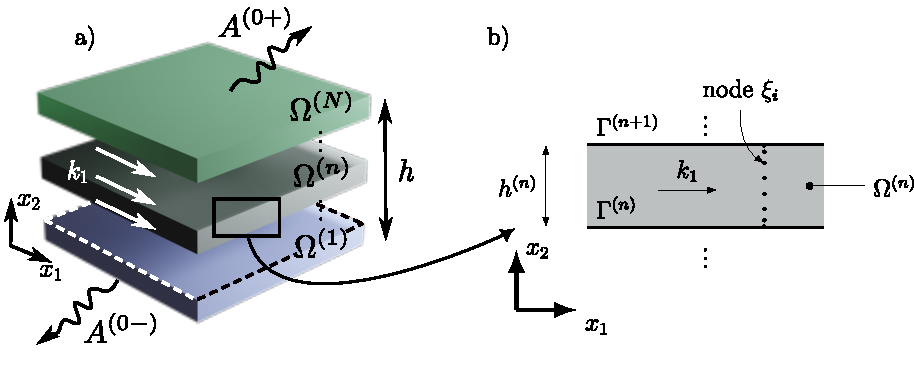
\includegraphics{chapitres/article_JAP/figures/fig1_schema.pdf}
    \caption{a) Sketch of the geometry of the multilayer system and b) zoom on the $n$-th layer.}
    \label{fig:schema_multilayer}
\end{figure}   
We assume an implicit time dependence $e^{-\im \omega t}$. The physical fields associated to the guided waves in the $n$-th layer propagating along the positive $x_1$-axis take the form
    \begin{equation}
         \boldsymbol{\Theta}^{(n)}  (\mbf x) = \mbf s^{(n)}(k_1,x_2) e^{\im k_1 x_1},
        \label{eq:field_ansatz}
    \end{equation}
where $\mbf s^{(n)}(k_1, x_2)$ is the spatial Laplace transform of $\boldsymbol{\Theta}^{(n)} (\mbf x)$ and $k_1$ is the complex valued $x_1$-component of the wavenumber. Note that the spatial Laplace transform is used instead of the spatial Fourier transform because $k_1$ is complex-valued.because $ k_1$, the $x_1$ component of the wavenumber is complex-valued. The physical fields that compose $\boldsymbol{\Theta}^{(n)}  (\mbf x)$ depend on the nature of the material occupying the $n$-th layer. Introducing $\boldsymbol{\Theta}^{(n)}  (\mbf x)$ in the corresponding wave equations (of second order in space in this work) reduces to a second-order differential operator $\mathcal L^{(n)}$ in $x_2$, that depends on the material properties and can further be developed as a second-order polynomial in $ k_1$
    \begin{equation}
        \mathcal L^{(n)}(x_2) \mbf s^{(n)}(k_1, x_2) = \left( k_1^2\mathcal L_2^{(n)}(x_2) + k_1\mathcal L_1^{(n)}(x_2) + \mathcal L_0^{(n)}(x_2) \right) \mbf s^{(n)}(k_1, x_2) = \mbf 0,
        \label{eq:operator_decomposition}
    \end{equation}
where $\mathcal L^{(n)}_j$ are the coefficients of the polynomial expansion $j=0,1,2$. Please note that this operator is nothing but the spatial Laplace transform of the equations of motion. 
    
The interface (boundary) conditions at $\Gamma^{(n)}$ between the $n+1$-th and the $n$-th layers again depend on the nature of these two layers, but can be formally written in the form
    \begin{equation}
        \mathcal C^{(n)-} \left. \mbf s^{(n)}(k_1) \right|_{\Gamma^{(n)}} - \mathcal C^{(n)+} \left. \mbf s^{(n+1)}(k_1) \right|_{\Gamma^{(n)}}= \mbf 0,
        \label{eq:coupling_operators}
    \end{equation}
 where $\mathcal C^{(n)\pm}$ are interfaces operators, which involve differential operators of maximum second-order in $x_2$. Following this procedure and introducing $\mbf S= \begin{pmatrix} \mbf s^{(0^-)}\ldots \mbf s^{(n)} \ldots \mbf s^{(0^+)} \end{pmatrix}^\transp$, with $^\transp$ denoting transposition, the problem can be cast in matrix form, whose coefficients are differential operators in $x_2$,
    \begin{equation} \mbf K \mbf S(k_1, x_2) = 
        \begin{pmatrix}
            \mathcal C^{(0^-)} & -\mathcal C^{(0^+)} & 0 & \\
            0 & \mathcal L^{(1)}(x_2) & 0 &  \\
            0 & \mathcal C^{(1^-)} & -\mathcal C^{(1^+)} & 0   & \\
            & 0 & \mathcal L^{(2)}(x_2)  & 0  & \\
            & & \ddots & \ddots & \ddots \\
            & & & 0 & \mathcal L^{(N)}(x_2)  & 0 \\
            & & & 0 & \mathcal C^{(N^-)} & -\mathcal C^{(N^+)}
        \end{pmatrix}\mbf S (k_1, x_2) = \mbf 0.
        \label{eq:op_k_matrix}
    \end{equation}
Note that the equations of motion in both upper and lower half-spaces are not required in Eq.(\ref{eq:op_k_matrix}). This system only depends on the values of the two spatial Laplace transforms $s^{(0^\pm)}$ at the upper and lower interfaces. Instead, we specify the nature of the two half-spaces, i.e. a fluid medium, and make use of the Sommerfeld condition, to explicitly give the form of the spatial Laplace transforms $\tilde{p}^{(0^\pm)}(k_1,x_2)$ of the pressure fields $p^{(0^\pm)}(\mbf x)$
    \begin{equation}
    \begin{array}{ll}
        \tilde{p}^{(0^-)}(k_1,x_2) &\displaystyle = A^{(0-)} e^{-\im  k_{2}^{(0)} x_2},  \in \Omega^{(0^-)},\\
        \tilde{p}^{(0^+)}(k_1,x_2) &\displaystyle= A^{(0+)} e^{\im  k_{2}^{(0)} (x_2 - h)}, \in \Omega^{(0^+)},\\
        \end{array}
        \label{eq:outgoing_pressure_field}
    \end{equation}
with $ k_{2}^{(0)}=\sqrt{\left(k^{(0)}\right)^2- k_1^2}$, such that $\textrm{Re}\left( k_{2}^{(0)}\right)\geq 0$, where $k^{(0)} = \omega /c_f$ is the wavenumber in the fluid and $c_f$ the wave velocity. Thus, $\mbf s^{(0^\pm)}$ appearing in  Eq.(\ref{eq:op_k_matrix}) reduces to $s^{(0^\pm)}=A^{(0\pm)}$. $\mathcal{C}^{(0^-)}$ and $\mathcal{C}^{(N^+)}$ are therefore no longer operators and reduce to $\mathcal{C}^{(0^-)}= \mbf C^{(0^-)}$ and $\mathcal{C}^{(N^+)}=\mbf C^{(N^+)}$. In our fluid case, the interface conditions at $\Gamma^{(0)}$ and $\Gamma^{(N)}$ involve the spatial Laplace transform of the pressure and its first spatial derivative with respect to $x_2$ whatever the nature of the $1$-st and $N$-th layers.  Both matrices $ \mbf C^{(j)}$, $j=(0^-),(N^+)$, can thus be formally written as
    \begin{equation}
        \mbf C^{(j)} = k_1 \mbf C_1^{(j)}+\mbf C_0^{(j)}+k_2^{(0)}\mbf C_{1'}^{(j)},
        \label{eq:continuity}
    \end{equation}
with the subscript denoting the submatrices rearranged according to the power order $k1$. Index $1'$ corresponds to the term in $k_2^{(0)}$. Introducing Eqs.(\ref{eq:operator_decomposition}) and (\ref{eq:continuity}) in Eq.~(\ref{eq:op_k_matrix}) leads to
    \begin{equation}
       \left(  k_1^2 \mbf K_2 +  k_1 \mbf K_1 + \mbf K_0 + \im k_2^{(0)} \mbf K_{1'} \right) \mbf S = \mbf 0.
       \label{eq:nl_gep}
    \end{equation}
This eigenvalue problem is non-linear because of the presence of the term $k_2^{(0)}$. Making use of the following changes of variable $ k_1 = k^{(0)} \left(\gamma + \gamma^{-1} \right)/2$ and $\ k_2^{(0)}= k^{(0)} \left(\gamma - \gamma^{-1} \right)/2i$ \cite{hood2017, betcke2013} and companion linearization \cite{gohberg2009}, a generalized eigenvalue problem is formed and solved for $\gamma$, from which the dispersion relation can be calculated. More details on this procedure can be found in \cite{kiefer2019}. 
Note that the first or the last column of Eq.(\ref{eq:op_k_matrix}) vanishes when radiation is absent on either side of the multilayer system. The situation is different when both fluid half-spaces disappear. The eigenvalue problem Eq.(\ref{eq:nl_gep}) is no longer non-linear and the problem can directly be solved after companion linearization. Note also that fluid half-spaces are only considered for the sake of simplicity and that this procedure can be adapted to any kind of material occupying the half-spaces, as described recently ~\cite{gravenkamp2024}. Note finally that this procedure avoids discretization of these two half-spaces.
    
To numerically solve the problem, the spatial Laplace transform of the physical fields in each $n$-th layer are expanded as
    \begin{equation}
        \mbf s^{(n)}(x_2) \approx \numvec s^{(n)}(x_2) = \sum_{m = 0}^M \alpha_m^{(n)} \numvec \psi_m (\xi^{(n)}),
        \label{eq:field_to_polynomial}
    \end{equation}
    where $\alpha_m$ are coefficients of the polynomial expansion, $\numvec \psi_m$ are the Chebyshev polynomial of order $m$, and $\xi^{(n)} = 2(x_2-\sum_{j=1}^{n-1}h^{(j)})/h^{(n)} - 1,~\in[-1,1]$. Underlined variables represent discrete vectors and double-underlined variables discrete matrices. The goal of this approximation is to discretize the differential operators in $x_2$ appearing in the problem. To do so, the SCM is employed. $\xi^{(n)}$ is discretized on the roots of the Chebyshev polynomials, $\numvec \xi_j^{(n)} = \cos\left(\frac{j\pi}{M^{(n)}}\right)$ with $j=0\ldots M^{(n)}$. Please note that $\numvec \xi_j^{(n)}$ discretely runs from 1 to -1 with increasing $j$, while $\xi^{(n)}$ continuously runs over the same interval but in the opposite direction, i.e. from -1 to 1. These collocation points/nodes form a non-uniform grid along the thickness of each layer. This discretization is usually preferred because the collocation points are clustered at the interfaces \cite{trefethen2000}. The locations of these nodes are presented in Fig.~\ref{fig:schema_multilayer}b for the $n$-th layer with an arbitrary value $M^{(n)}=8$. The differential operators in the $n$-th layer are thus represented by differentiation matrices (DMs), such that
    \begin{equation}
        \begin{aligned}
            \mbf s^{(n)} (x_2) & \rightarrow \nummat I \:\numvec s^{(n)} (\numvec\xi_j), \quad \quad
            \partial_2 \mbf s^{(n)} (x_2) \rightarrow \left( \frac{ 2}{ h^{(n)}} \right) \nummat{ D_2} \: \numvec s^{(n)}(\numvec \xi_j)= \nummat{ D_2}^{(n)} \: \numvec s^{(n)}(\numvec \xi_j), \\
            & \partial_{22} \mbf s^{(n)} (x_2) \rightarrow \left( \frac{ 2}{ h^{(n)}} \right)^2 \nummat D_{22} \:\numvec s^{(n)}(\numvec \xi_j)= \nummat D_{22}^{(n)} \:\numvec s^{(n)}(\numvec \xi_j). \\
        \end{aligned}
        \label{eq:diff_matrices}
    \end{equation}
where $\nummat I$ is the identity matrix and $\nummat D_2$ and $\nummat D_{22}$ are respectively the first-order and second-order normalized DMs. Contrary to an interpolation with Chebyshev polynomials, DMs interpolate the functions and their spatial derivatives directly and thus do not involve the polynomial expansion coefficients per se.~\cite{weideman2000}. Note that the normalized DMs are denoted as $\nummat D_{2}^{(n)}$ and $\nummat D_{22}^{(n)}$ in the following . These matrices are square and have a size of $(M \times M)$. This size also directly depends on the order of the considered Chebyshev polynomials. The formulation prevents the occurrence of roundoff errors, which is of particular importance when SCM is applied to solve eigenvalue problems \cite{baltensperger2003}.
    
The linear operator $\mathcal L^{(n)}$ is discretized as a matrix $\nummat L^{(n)}$ with size $(P^{(n)} (M^{(n)} - 1), P^{(n)} (M^{(n)} + 1))$, where $P^{(n)}$ is the number of physical fields required to describe the wave propagation in the layer and again depends on the nature of the material this layer is composed of. The first and the last rows of the DMs are removed because they are used to apply the interface conditions at $\Gamma^{(n+1)}$ and $\Gamma^{(n)}$ respectively. The interface operators $\mathcal C^{(n)\pm}$ are effectively expressed in terms of this first row of the DMs of the $n$-th layer and this last row of the DMs of the $(n+1)$-th layer. These rows respectively correspond to the first, i.e. $\numvec\xi_{M^{(n)}}=-1$ and $\xi^{(n)}=1$, and last collocation nodes of the $n$-th and $(n+1)$-th layers, i.e. $\numvec\xi_0=1$ and $\xi^{(n+1)}=-1$.  These vectors are subsequently denoted $\numvec I^{(n+1)-}$, $\numvec I^{(n)+}$, $\numvec D_{2}^{(n+1)-}$, $\numvec D_{2}^{(n)+}$, $\numvec D_{22}^{(n+1)-}$, and $\numvec D_{22}^{(n)+}$. The interface matrix $\nummat C^{(n)^-}$ is of size $(P^{(n)}+P^{(n+1)},P^{(n)}(M^{(n)}+1))$ and the interface matrix $\nummat C^{(n)^+}$ is of size $(P^{(n)}+P^{(n+1)},P^{(n+1)}(M^{(n+1)}+1))$.
    
Finally, the full $(\sum_{n=0}^N M^{(n)} P^{(n)} + 2,\sum_{n=0}^N M^{(n)} P^{(n)} + 2)$-matrix  system for the general multilayer system is
    \begin{equation} \nummat K \: \numvec S = 
        \begin{pmatrix}
            \nummat C^{(0^-)} & -\nummat C^{(0^+)} & 0 & \\
            0 & \nummat L^{(1)} & 0 &  \\
            0 & \nummat C^{(1^-)} & -\nummat C^{(1^+)} & 0   & \\
            & 0 & \nummat L^{(2)}  & 0  & \\
            & & \ddots & \ddots & \ddots \\
            & & & 0 & \nummat L^{(N)}  & 0 \\
            & & & 0 & \nummat C^{(N^-)} & -\nummat C^{({N}^+)}
        \end{pmatrix}
        \begin{pmatrix}
                A^{(0-)} \\ \numvec s^{(1)} \\ \numvec s^{(2)} \\ \vdots \\ \numvec s^{(N)} \\ A^{({0+})} 
        \end{pmatrix} = \numvec 0.
        \label{eq:discretized_multilayer_system}
    \end{equation}
    
This system is cast in the form of a generalized eigenvalue problem that is solved by traditional eigenvalue solvers at each frequency. The dispersion relation for the acoustic guided wave in the dissipative multilayer system is calculated, repeating the procedure for each frequency $\omega$.
    
\subsection{Solving the dispersion relation with M\"uller algorithm}
    \label{subsec:semi_a}

The dispersion relation of multi-layer dissipative structure are more commonly calculated with secant-based algorithm as the M\"uller algorithm. The latter relies on a semi-analytic description of the fields. These fields are best written in each layer, independently of the nature of the material it is composed of, using the potentials, i.e. decomposing the field $\mbf \theta = \mbf \nabla \varphi + \mbf \nabla \times \mbf \psi$ into an irrotational component $\varphi$ and a transverse component $\mbf \psi=\psi \mbf e_3$. The spatial Laplace transform of the potentials in the $n$-th layer are entirely described by
    \begin{equation}
        \tilde { \mbf \theta}_n ( k_1, x_2) =  A^{(n)+}_{X} e^{\im  k_{2,X}^{(n)}(x_2 - h^{(n)})} + A^{(n)-}_{X} e^{-\im  k_{2,X}^{(n)} (x_2 - h^{(n)})}, 
    \end{equation}
with $ A^{(n)\pm}_{X}$ the up and down-going wave amplitudes, $k_{2,X}^{(n)}=\sqrt{\left(k_{X}^{(n)}\right)^2-k_1^2}$, such that $\textrm{Re}\left( k_{2,X}^{(n)}\right)\geq 0$, and $X$ refers to the type of wave, i.e. shear, compressional or acoustic. If necessary, these Laplace transform representations are complemented by those of the pressure field in the fluid half-spaces provided in Eq.(\ref{eq:outgoing_pressure_field}).

The boundary conditions are applied at each interface and the set of equations is cast into the following matrix form $\mbf M( k_1) \mbf q = 0$, with $ \mbf q$ a vector containing the amplitudes of each field/potential. The modes of the system correspond to the wavenumbers $ k_1$ for which the matrix $\mbf M( k_1)$ is singular, i.e.
    \begin{equation}
        \text{det}\left( \mbf M( k_1)\right) = 0.
        \label{eq:det_M}
    \end{equation}
These wavenumbers are the complex roots of an implicit complex-valued equation. They are evaluated by running our own implementation of the Müller algorithm \cite{muller1956} from 3 initial guesses. This equation is solved iteratively for each frequency $\omega$, giving the dispersion relation.
    
In addition, $\mbf q$ can be obtained by computing the nullspace of $\mbf M$ \cite{strang2022} (This null space is computed using singular value decomposition as embedded in the \texttt{linalg.null\char`_space} function from the Python package SciPy). The amplitudes of the potentials in the layers are thus evaluated, enabling all the physical fields that depend on these potentials to be calculated. However, the $\mbf M$ matrix becomes increasingly tedious to write as the number of layers increases, and even more so when it comes to calculating the roots of its determinant and nullspaces. Nevertheless, this approach remains a fairly effective way of providing a reference solution for validating numerical results when studying a two-layer system.
    
%%%%%%%%%%%%%%%%%%%%%%%%%%%%%%%%%%%%%%%%%%%%%%%
\section{Application to a two-layer poroelastic-elastic structure}\label{Section3}

 In this section, the calculation of the dispersion relation for guided waves in a two-layer structure, i.e. $N=2$, is used as an example of the application of the present SCM. This two-layer structure consists of a $h^{(1)}$-thick poroelastic layer, coated on one side by a $h^{(2)}$-thick aluminum plate,  that is radiating in a fluid half-space, and rigidly backed on the other side as depicted in Fig.~\ref{fig:bilayer}a. The SCM results are analyzed and compared to those obtained with the Müller root-finding method. 

    %As a preliminary step, the dispersion relation for guided waves in a single $2h^{(1)}$-thick poroelastic plate with both sides coupled to the same fluid half-spaces is detailed in the appendix \ref{app:fluid_coupled_poroelastic}. To facilitate the dispersion relation analysis, the poroelastic thickness is twice that considered in the two-layer structure. Effectively, the rigid boundary acts as a mirror symmetry plane.
    
\subsection{Numerical scheme}
The pressure field $p^{(1)}$ and the two components of the frame displacement, $u_{1, s}^{(1)}$ and $u_{2,s}^{(1)}$, i.e. $P^{(1)} = 3$, as well as the two-components of the elastic displacement, $u_1^{(2)}$ and $u_2^{(2)}$, i.e. $P^{(2)} = 2$, are used to model the propagation in the poroelastic and in the elastic layers respectively. The $\{\mathbf{ u}_s, p \}$ formulation is used~\cite{atalla1998} for the poroelastic medium. The more usual displacement formulations ($\{\mathbf{u}_s, \mathbf{u}_f\}$\cite{biot1956} or $\{\mathbf{u}_s, \mathbf{w}\}$~\cite{biot1962}) cannot be used in the present case, because the number of physical fields they rely on, i.e. 4, is different from that of the potentials in the layer, i.e. 3.


% instead of the more classical formulations.
% Although these formulations are formally equivalent for homogeneous and isotropic poroelastic materials, the latter two consist of a set of 4 equations. They use a fourth degree of freedom, whereas there are only 3 physical potentials, hence the choice of a formulation consisting of a set of $3$ equations of motion governing $3$ fields. 

In total, 5 physical fields inside the two-layer structure and an additional amplitude for the acoustic wave radiated towards $x_2 \rightarrow \infty $ are needed to solve for the dispersion relation. Each domain is discretized on $M^{(j)}$, $j=1,2$, collocation points.

In more details, the $\{\mbf u_s, p\}$ formulation of the Biot theory \cite{atalla1998} is employed to model the propagation in the homogeneous isotropic poroelastic layer. The coupled equations of motion read as
    \begin{equation}
        \left\{
        \begin{aligned}
            \nabla \cdot \mbf{\hat{\sigma}}_s^{(1)} + \hat \rho \omega^2 \mbf u_s^{(1)} +  \beta \mbf \nabla p^{(1)} &= 0, \\
            \frac{\nabla^2 p^{(1)}}{\rho_{22} \omega^2} - \frac{\beta}{\phi^2} \nabla \cdot \mbf u_s^{(1)} + \frac{1}{ R}p^{(1)} &= 0,
        \end{aligned}
        \right.
        \label{eq:up_motion_equations}
    \end{equation}
    where $\mbf{\hat{\sigma}}_s^{(1)} = \hat A \nabla \cdot \mbf u_s^{(1)} \mbf I + 2 N_s \mbf \varepsilon_s$ is the \emph{in vacuo} solid stress tensor, with $\mbf \varepsilon_s$, the solid-phase strain tensor. The parameters are generally expressed in terms of the elastic coefficients $ P$,  $Q$ and $ R$ and the effective densities $\rho_{11}, \rho_{12}$ and $ \rho_{22}$ initially introduced by Biot~\cite{biot1956,allard2009} as
    \begin{equation}
        \begin{split}
             \hat A = P-2N_s - \frac{ Q^2}{ R}, \quad \hat \rho = \rho_{11} - \frac{ \rho_{12}^2}{ \rho_{22}},
            \quad \beta = \phi \left( \frac{ \rho_{12}}{ \rho_{22}} - \frac{ Q}{ R} \right).
        \end{split}\label{eq:biot_coefs}
    \end{equation}
These parameters depend on the frame properties and on the effective density ${\rho}_{eq}(\omega)$ and bulk modulus ${K}_{eq}(\omega)$ of the fluid phase as reminded in \ref{app:coefs}. In short, a poroelastic material is entirely described by the porosity $\phi$, the shear modulus of the frame $N_s$, the Poisson ratio $\nu$, the density of the frame $\rho_1$, the viscous and thermal characteristic lengths $\Lambda$ and $\Lambda'$, tortuosity $\alpha_\infty$, and the flow resistivity $R_f$ when saturated by a light fluid~\cite{biot1956,johnson1987,champoux1991}. All these parameters are real valued except for the shear modulus, which incorporates a viscoelastic damping factor.
    
Introducing $ \mbf s^{(1)} =(\tilde u_1^s, \tilde u_2^s, \tilde p )^\transp$, the spatial Laplace transform of Eq.~(\ref{eq:up_motion_equations}) is expanded in the form of Eq.~(\ref{eq:operator_decomposition}) with
    \begin{equation}
        \begin{array}{l}
        \mathcal L_0^{(1)} =
            \begin{pmatrix}
                 N_s \partial_{22} + \hat \rho\omega^2 & 0 & 0 \\
                0 & \hat P \partial_{22} +\hat \rho\omega^2 & \beta \partial_2 \\
                0 & -\beta/\phi^2\partial_2 & 1/ R + \partial_{22}/( \rho_{22}\omega^2) 
            \end{pmatrix},\\[24pt]
        \mathcal L_1^{(1)} = 
            \begin{pmatrix}
                0 & \im\hat P \partial_2 & \im \beta \\
                \im(\hat A + N_s) \partial_2 & 0 & 0 \\
                -\im\beta/\phi^2 & 0 & 0 \\
            \end{pmatrix},\textrm{ and }
                 \mathcal L_2^{(1)}  = 
            \begin{pmatrix}
                \hat P & 0 & 0 \\
                0 &  N_s & 0 \\
                0 & 0 & 1/( \rho_{22} \omega^2)
            \end{pmatrix}.
        \end{array}
        \label{eq:up_motion_equations_decomposed}
    \end{equation}
    
Finally, the discretized equations of motion read as
    \begin{equation}   
        \nummat L^{(1)} \numvec s^{(1)} = \begin{pmatrix}
            (\omega^2 \hat \rho - k_1^2 \hat P) \nummat I +  N_s \nummat D_{22}
            & \im  k_1 (\hat P -  N_s) \nummat D_{22} 
                & -\im k_1 \beta \nummat I \\
                \im  k_1 (\hat P -  N_s) \nummat D_2 
                & \hat P \nummat D_{22} +(\omega^2 \hat \rho -  k_1^2   N_s) \nummat I
                & \beta \nummat D_2 \\

                \displaystyle \frac{-\im  \beta \omega^2}{\phi^2} \nummat I &\displaystyle \frac{-\beta \omega^2}{\phi^2} \nummat D_2 & 
                \displaystyle \frac{ k_1^2}{ \rho_{22}} \nummat I + \displaystyle \frac{\omega^2}{ R} \nummat I

                % -\im k_1 \tilde \gamma \nummat I 
                % & -\tilde \gamma \nummat D_2
                % & \left(\frac {\phi^2}{\tilde R} -\frac{\phi^2 k_1^2}{\tilde\rho_{22} \omega^2} \right)\nummat I 
            \end{pmatrix} \numvec s^{(1)} = 0. 
            \label{eq:up_motion_equations_discrete}
        \end{equation}
    
The equation of motion in the elastic medium is derived from the fundamental elasticity equations \cite{achenbach2014} and reads as, 
    \begin{equation}
        \rho \omega^2 \mbf u^{(2)} + (\lambda + \mu) \mbf{\nabla}(\nabla \cdot \mbf u^{(2)} ) + \mu\nabla^2 \mbf u^{(2)} = 0,
    \label{eq:elastodynamic}
    \end{equation}
where $\rho$ is the density and $\lambda$ and $\mu$ are the Lam\'e coefficients.
The corresponding discretized equation of motion is
        \begin{equation}
             \nummat L^{(2)} \numvec s^{(2)} =\left(\frac{\rho^{(2)}}{\mu} \omega^2 \nummat I +
            \begin{pmatrix}
                - k_1^2(\lambda / \mu + 2) \nummat I + \nummat D_{22}& \im  k_1 (\lambda / \mu + 1) \nummat D_2 \\
                \im  k_1 (\lambda/ \mu + 1) \nummat D_2 & (\lambda / \mu + 2)\nummat D_{22} - k_1^2 \nummat I
            \end{pmatrix} \right) \numvec s^{(2)} = 0.
            \label{eq:elastodynamic_discrete}
        \end{equation}
    
The interface and boundary conditions depend on the vectors $\numvec I^\pm, \numvec D_{2}^\pm$ and $\numvec D_{22}^\pm$ which corresponds to the last (subscript $+$) and first row (subscript $-$) of the DMs. From the bottom to the top of the two-layer system, they are
        \begin{itemize}
        \item Rigid boundary condition at $\Gamma^{(0)}$ which leads to
        \begin{equation}
            \mbf u^{(1)}(x_2=0) = 0; \quad 
            \mbf u_f^{(1)}(x_2=0) \cdot \mbf n - \mbf u_s^{(1)}(x_2=0) \cdot \mbf n = 0,
            \label{eq1}
    \end{equation}
the discretized form of which is,
    \begin{equation} \nummat C^{(0)} \numvec s^{(1)} = 
        \begin{pmatrix}
            \numvec 0 & \numvec I^+ & \numvec 0 \\
            \numvec 0 & \numvec 0 & \numvec I^+ \\
           \displaystyle \frac{\phi}{ \rho_{22} } \numvec D_{2}^+ & \numvec 0 & - \left( 1 +\displaystyle\frac{ \rho_{12}} { \rho_{22}} \right) \omega^2\numvec I^+
        \end{pmatrix} \begin{pmatrix}
            \numvec p^{(1)} \\ \numvec u^{(1)}_{1} \\ \numvec u^{(1)}_{2}
        \end{pmatrix} = \numvec 0.
        \label{eq:rigid_poro_cont_matrix}
    \end{equation}
    \item Continuity between the poroelastic and the elastic media~\cite{debergue1999} at $\Gamma^{(1)}$ which leads to
    \begin{equation}
    \begin{array}{c}
          \mbf \sigma^{t(1)}(x_2=h^{(1)})-\mbf \sigma^{(2)}(x_2=h^{(1)})=0; \quad 
        \mbf u^{(2)}(x_2=h^{(1)}) = \mbf u_s^{(1)}(x_2=h^{(1)}); \\
        \mbf u_f^{(1)}(x_2=h^{(1)}) \cdot \mbf n - \mbf u_s^{(1)}(x_2=h^{(1)}) \cdot \mbf n = 0,
        \end{array}
    \end{equation}
   where $\mbf \sigma^{t(1)} = \hat{\mbf \sigma_s} - \phi \left( 1 + Q/R\right)$ is the total stress tensor in the poroelastic layer. The corresponding discretized interface matrices, arising from 
    \begin{equation}
        \nummat C^{(1)+} \numvec s^{(2)} - \nummat C^{(1)-} \numvec s^{(1)} =
        \nummat C^{(1)} \begin{pmatrix} \numvec p^{(1)} & \numvec u^{(1)}_{1} & \numvec u^{(1)}_{2} & \numvec u^{(2)}_{1} & \numvec u^{(2)}_{2}
        \end{pmatrix}^\transp = 0,
    \end{equation}
    are cast as
    \begin{equation} \nummat C^{(1)}  = 
       \left(
        \begin{array}{ccc|cc}
            - N_s\numvec D_{2}^+ & -\im  k_1  N_s \numvec I & \numvec 0 & \mu \numvec D_{2}^- & \im  k_1 \mu \numvec I^- \\
            -\im  k_1 \hat A \numvec I^+ & -\hat P \numvec D_{2}^+ & \phi \left(1 + \cfrac{ Q}{ R}\right) \numvec I^+ & \im  k_1 \lambda\numvec I^- & (\lambda + 2\mu )\numvec D_{2}^-  \\
            \numvec 0 & -\numvec I^+ & \numvec 0 & \numvec I^- & \numvec 0  \\
            \numvec 0 & \numvec 0 & -\numvec I^+ & \numvec 0 & \numvec I^-  \\
            -\cfrac{\phi}{ \rho_{22}} \:\numvec D_{2}^+ & \left( 1 +\displaystyle\frac{ \rho_{12}} { \rho_{22}} \right)\omega^2\numvec I^+ & \numvec 0 & \numvec 0 & \numvec 0 \\
        \end{array} \right),
        \label{eq:poro_elastic_cont_matrix}
    \end{equation}
    with the left-hand side corresponding to $\nummat C^{(1)-}$ and the right-hand side to $\nummat C^{(1)+}$.
    \item Continuity between the elastic and the fluid media at $\Gamma^{(2)}$ which leads to
    \begin{equation}
    \begin{array}{c}
            \sigma_{12}^{(2)}(x_2=h) = 0; \quad \quad \sigma_{22}^{(2)}(x_2=h) = -p^{(0+)}; \\ 
             u_2^{(2)}(x_2=h)=u_2^{(0+)}(x_2=h).
             \end{array}
    \end{equation}
    The corresponding discretized interface matrix $\nummat C^{(2)} \begin{pmatrix} \numvec u^{(2)}_1 & \numvec u^{(2)}_2 & A^{(0+)}\end{pmatrix}^\transp = 0$ is 
        \begin{equation} \nummat C^{(2)} = 
            \left( \begin{array}{cc|c}
                    \numvec D_{2}^+ & \im  k_1 \numvec I^+ & 0 \\
                    \im  k_1 \lambda \numvec I^+ & (\lambda + 2\mu)\numvec D_{2}^+ & 1 \\
                    \numvec 0 & \omega^2 \numvec I^+ & \cfrac {\im k_2^{(0)}}{\rho_f}
                \end{array} \right).
            \label{eq:elastic_fluid_cont_matrix}
        \end{equation}
    \end{itemize}
    
Combining the discretized interface conditions, Eqs.(\ref{eq:rigid_poro_cont_matrix}), (\ref{eq:poro_elastic_cont_matrix}) and, (\ref{eq:elastic_fluid_cont_matrix}), with the discretized equations of motion, Eqs.(\ref{eq:up_motion_equations_discrete}) and (\ref{eq:elastodynamic_discrete}), leads to the following system
    \begin{equation}
        \begin{pmatrix}
            \nummat C^{(0)} & 0 & 0 \\[1ex]
            \nummat L^{(1)} & 0 & 0 \\[1ex]
            \nummat C^{(1)-} & -\nummat C^{(1)+} & 0 \\[1ex]
            0 & \nummat L^{(2)}  & 0 \\[1ex]
            0 & \nummat C^{(2)-} & -\nummat C^{(2)+} \\[1ex]
        \end{pmatrix}
        \begin{pmatrix}
                \numvec s^{(1)} \\ \numvec s^{(2)} \\ A^{(0+)} 
        \end{pmatrix} = \numvec 0.
    \end{equation}
This system is further expanded in the form of Eq.(\ref{eq:nl_gep}) and solved for a set of eigenvalues $\gamma$ and associated eigenvectors $\mbf S$ at each frequency $\omega$. Wavenumbers $ k_1$ are then obtained from $\gamma$. The dispersion curve is thus calculated over a given frequency range. However, the condition $\textrm{Re}\left(k_2^{0}\right)\geq0$ should be imposed to sort out the solution that do not meet it.

Although usual and simple, this two-layer structure is challenging from a numerical point of view because it involves materials with very large impedance contrasts and layers whose thicknesses differ by several orders of magnitude. These problems are partially solved by normalizing each line and rearranging the terms of the matrix Eq.~(\ref{eq:nl_gep}), leading to a better numerical conditioning of the system. 
    
    \begin{figure}
        \centering
        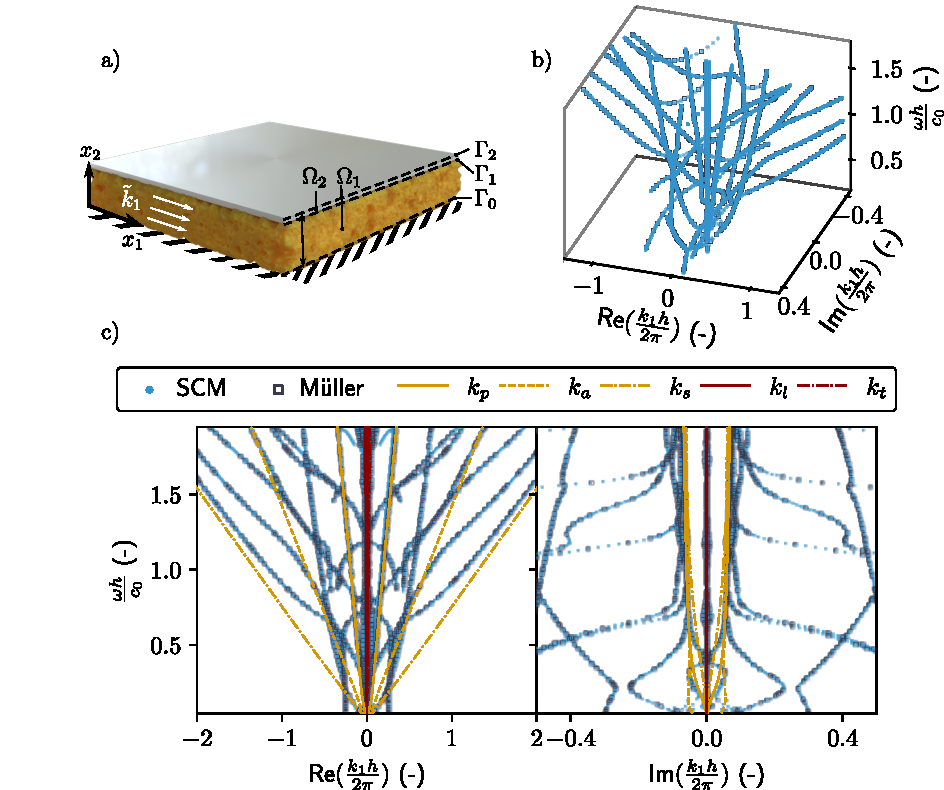
\includegraphics{chapitres/article_JAP/figures/bicouche.pdf}
        \caption{ a) Sketch of the two-layer structure geometry. b) 3D view of the complex wavenumber-real frequency dispersion relation and c) real and imaginary parts of the dispersion relation. Blue dots represents the results as calculated with the SCM and black open markers represents those as calculated with the Müller method. Bulk wavenumbers in the poroelatic and elastic materials are highlighted in yellow and dark red respectively.}
        \label{fig:bilayer}
    \end{figure}
    
    \subsection{Dispersion relation}\label{Disrel}
The material properties of the $h^{(1)}= 52\textrm{ mm}$-thick poroelastic (melanime) layer are listed in Table~\ref{tab:poroelastic_params}, while the properties of the $h^{(2)}=1\textrm{ mm}$-thick aluminium plate are the density $\rho = 2700 \textrm{ kg.m}^{-3}$ and the Lamé coefficients $\lambda = 60.75 \textrm{ GPa}$ and $\mu =  26.03 \textrm{ GPa}$. The saturating fluid and that occupying the half-space is air with density $\rho_f = 1.213\textrm{ kg.m}^{-3}$, the heat capacity ratio $\kappa = 1.4$, kinematic compressibility $\mu_f = 1.839 \times 10^{-5} \textrm{ Pa.s}$, the Prandtl number $\textrm{Pr} = 0.71$, and adiabatic bulk modulus $\kappa P_0$, where the atmospheric pressure is $P_0 = 1.013 \times 10^5 \textrm{ Pa}$. The total two-layer thickness is thus $h=h^{(1)}+h^{(2)}=53\textrm{ mm}$. $M^{(1)}=5$ and $M^{(2)}=11$ collocation points are employed respectively in the poroelastic and elastic layers.
    
The 3D view of the complex dispersion diagram is depicted Fig.~\ref{fig:bilayer}b. To ease readability, real and imaginary parts are depicted separately in Fig.~\ref{fig:bilayer}c. Please note that this last representation can be misleading because only the modes that lie in the complex wavenumber range depicted in Fig.~\ref{fig:bilayer}b are represented in Fig.~\ref{fig:bilayer}c. Cut-on frequencies are thus fictitious. The results calculated using the SCM method, plotted in blue markers, are compared with those obtained using the M\"uller method, plotted with black open markers. Both methods provide identical results, up to around four digits, therefore validating the present approach. Note that the SCM solutions are used as initial guesses of the M\"uller algorithm to shorten computational time. In this way, fewer iterations are needed for the results of the root-finding method to converge. The main advantages of SCM are that no initial guesses are needed, i.e. as long as the discretization is sufficient to model the full wave behavior in the structure, the dispersion relation is guaranteed to be calculated. In addition, the matrices used for the numerical model are very small compared to those required by other methods such as FEM, and are therefore much less demanding in terms of calculation.
    \begin{table}
        \centering
             \caption{Parameters of the poroelastic material (melamine foam)}
        \label{tab:poroelastic_params}

            \begin{tabular}{cccccccccc}
            \hline
            Parameter  & $\phi$ & $\rho_1$    & $R_f$          & $\Lambda$ & $\Lambda'$ & $\alpha_\infty$ & $\nu$  & $N_s$    \\
            Unit       & -      & kg.m$^{-3}$ & kPa.s.m$^{-2}$ & $\mu$m    & $\mu$m     & -               & -      & kPa            \\
            \hline
            Melamine   & $0.98$ & $6.5$       & $5.6$          & $214$     & $214$      & $1$             & $0.24$ & $11.96\left(1+\textrm{i0.07} \right)$     \\
            \hline
        \end{tabular}\\[2em]        
        \end{table}

    Wavenumbers are perfectly symmetric with both $\textrm{Re}\left(k_1h/2\pi \right)=0$, and $\textrm{Im}\left(k_1h/2\pi \right)=0$ axis, which is a feature of reciprocal systems. Wavenumbers having a very large slope and a low imaginary part correspond to modes mostly propagating in the aluminium plate. They are very close to the bulk longitudinal $k_l$ and tranverse $k_t$ wavenumbers in the aluminum. This is due to the very large contrast between the elastic properties of the aluminum and those of the poroelastic frame. The other branches asymptotically tend toward the bulk acoustic, $k_a$, compression, $k_p$, or shear, $k_s$, wavenumbers of the poroelastic medium at high frequency. At low frequencies, these modes are highly dispersive. 
    
    If we compare these results with the dispersion relation depicted in \ref{app:fluid_coupled_poroelastic}c) for the guided waves in a single poroelastic plate twice as thick and in the absence of the elastic plate, we find some essential differences . The branches associated with the elastic plate and the branch clearly associated with the coupling between the elastic and poroelastic layers (referenced as (1) in Fig.\ref{app:fluid_coupled_poroelastic}c)) do not exist. The other branches are similar to those of this single poroelastic layer, although slightly modified by the presence of the elastic plate. This proves a weak coupling between the elastic and poroelastic layers, particularly at high frequencies. At lower frequencies, the coupling between the two layers is stronger. Effectively, the wavelength is much larger than the thickness of at least one of the two layers in these frequency ranges, which favors coupling. The $A_0$ branch observed in the case of a single poroelastic layer disappear in the two-layer system rigidly backed, because this rigid-backing does not allow the existence of such a mode.
    
    \subsection{Mode shapes and energy fluxes}
    \label{sec:results_shapes}
    Beyond the SCM numerical efficiency, a significant advantage of the method is that the eigenvectors associated to each eigenvalue directly provides the associated mode shape. Since these mode shapes, i.e. eigenvectors, are calculated from an eigenvalue problem, their amplitude are defined up to a constant. They are normalized to the value of the pressure field at the bottom of the poroelastic layer, i.e. at the location of the rigid backing, because this condition imposes $\tilde{\mbf u}^{(1)}(0) = 0$ (and in particular $\tilde{u}_2^{(1)}(0) = 0$), which is equivalent to a maximum pressure field. From these normalized eigenvectors, any physical fields can be calculated as detailed in \ref{app:fields}.   

Let us consider two solutions $\ k_{1}^\pm=\pm |\textrm{Re}\left(k_{1}\right)|$ symmetric in the dispersion diagram with respect to the axis $\textrm{Re}\left(k_1 \right)=0$ as shown in Figs.~\ref{fig:results}a-b. The displacement fields and total energy fluxes in each direction are depicted in Fig.~\ref{fig:results}c-f. The results calculated using the SCM method, plotted in continuous lines, match those obtained using the Müller method, plotted with marker lines. These two modes are identical but propagate in opposite directions, i.e., the mode $ k_{1}^+$ propagates towards positive $x_1$ while the mode $ k_{1}^-$ propagates towards negative $x_1$. Displacement fields and energy fluxes are identical along the $x_2$ axis but are of equal modulus but opposite sign along the $x_1$ axis (see Fig.~\ref{fig:results}c-d and e-f). Both displacement field and energy flux amplitudes are two to three orders of magnitude smaller in the elastic plate (for $h_1<x_2<h$) than in the poroelastic plate. The aluminum coating is almost acting as a rigid boundary condition, as also testified by the fact that the $x_1$ components of the displacement field and energy fluxes are almost symmetric with respect to the axis $x_2=h_1/2$, while their $x_2$ components are almost antisymmetric along the $x_2$ axis. Note that the fluid phase Poynting vectors depicted in Fig.~\ref{fig:results}f are of equal modulus but opposite sign, symmetric with respect to the axis $x_2=h_1/2$, and more than a hundred times smaller than total energy flux in amplitude. The energy of these modes are thus mainly localized in the solid phase of the poroelastic plate. 
 
    \begin{figure}
        \centering
        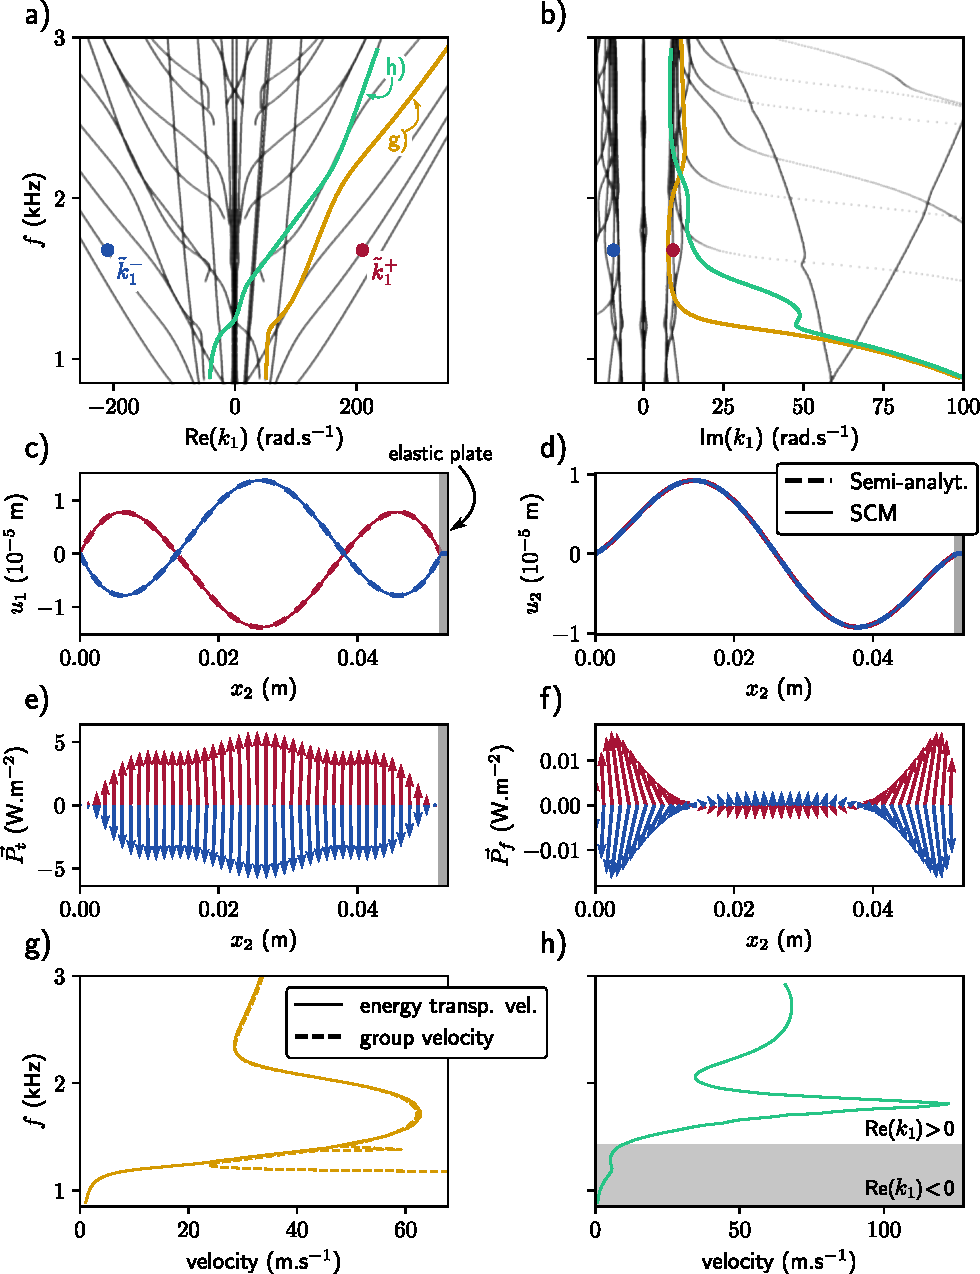
\includegraphics[scale=.9]{chapitres/article_JAP/figures/mode_shapes.pdf}
        \caption{a) and b) represent the real and imaginary parts of the dispersion relation of the two-layer structure. Two branches are highlighted in yellow and green, as well as two specific solutions (blue and red) symmetric with respect to the $\textrm{Re}\left( k_1\right)=0$ axis. Displacement fields in the $x_1$ (c) and $x_2$ direction d) associated with the forward (red) and backward (blue) solutions displayed above. e) Total Poynting vector and f) fluid Poynting vector in the poroelastic material distributions along the thickness of the structure for these two specific solutions. g) Group and energy transport velocities for the yellow branch. h) Energy transport velocity for the green branch. The gray area represents the frequency range over which this velocity is negative.}
        \label{fig:results}
    \end{figure}

    To go a step further, we evaluated the energy transport velocity $\overline{V_e} = \overline{P}_t / \overline U$ as the ratio between the average energy flux in each layer  $\overline{P}_t$ over the mean total energy $\overline U$. The energy transport velocity of the mode highlighted in orange in Fig.~\ref{fig:results}a-b is compared to the group velocity $v_g=\partial \omega/\partial \textrm{Re}\left(k_1 \right)$\cite{brillouin1946} in Fig.~\ref{fig:results}g. It is numerically computed by doing finite differences on a branch of the dispersion relation. Both velocities match for frequency ranges where the imaginary part of $ k_1$ is low, i.e., for weak attenuation modes~\cite{bernard2001,simonetti2005,castaings2003,carcione1996}, but are different for strong attenuation. In particular, the group velocity diverges around the cut-on frequency. This is the reason why the energy transport velocity is usually preferred to study absorbing structures. The energy transport velocity $\overline{V_e}$ of the mode highlighted in green Fig.~\ref{fig:results}a-b is depicted in Fig.~\ref{fig:results}h. This energy transport velocity is always positive, while $ k_1$ crosses the $\textrm{Re}\left(k_1 \right)=0$ axis. When 
    $\textrm{Re}\left(k_1 \right)<0$ the phase velocity is negative, while the $\overline{V_e}>0$. This branch (and the symmetric one) has also a negative group velocity as also testified by the fact $\textrm{Re}\left(k_1 \right)<0$ while $\textrm{Im}\left(k_1 \right)>0$  in the shaded area in Fig.~\ref{fig:results}h. This branch has also an exponentially growing amplitude.
    
%%%%%%%%%%%%%%%%%%%%%%%%%%%%%%%%%%%%%%%%%

    \subsection{Experimental validation}

The experimental set-up is depicted in Fig.~\ref{fig:expe}a. The sample is the two-layer structure considered in the previous subsection. The aluminum plate is glued on top of the poroelastic layer. The latter layer is glued on a $3\textrm{ cm}$-thick aluminium plate, which mimic the rigid backing. The three elements are $45\textrm{ cm}$ wide and $85 \textrm{ cm}$ long. The surrounding medium and the saturating fluid is air, at regular pressure and temperature conditions. The sample is positioned perpendicularly to the ground on its longest side as depicted in Fig.~\ref{fig:expe}a to ease the mode excitation in the poroelastic layer. The excitation is provided by a shaker (Brüel and Kjaer type 4810), which is rigidly attached to the sample with a threaded steel rod fixed to the shaker on one side and glued on a $1 \textrm{mm}$ thick aluminum plate of width $10 \textrm{ cm}$ and height $1.5 \textrm{ cm}$. This plate is cut at the edge opposite to the threaded steel rod and glued to the porous sample, creating a line source at the edge of the sample. The resonance of this part was measured to be 4500 Hz, which is the upper limit of the measured frequency range. The excitation signal is a swept-sine function with 400 points ranging from $1 \textrm{ kHz}$ to $3 \textrm{ kHz}$. The general layout of the experiments is similar to that used originally in \cite{geslain2016}. The key difference in our case is that the excitation is operated directly to the poroelastic layer and not to the top of the aluminum plate, because the modes that corresponds to propagating solutions in the poroelastic layer are encapsulated in between two almost rigid plates (see Section \ref{sec:results_shapes}). The normal displacement is measured with a laser Doppler vibrometer (Polytec VibroFlex Neo) on a line of length $L = 40$ cm, along the side of the thickness of the porous layer. These measurements are averaged 100 times. The excitation signal and the measured field are interfaced through a computer via a Zürich Instruments acquisition card. 

The SLaTCoW method \cite{geslain2016} is used to analyze the space-frequency displacement measurements and recover the complex wavenumber-real frequency dispersion relation. This method relies on the Laplace spatial transform of these measurements, which gives access to the real and imaginary components of the complex wavenumber. The difference between this Laplace transform and a correctly chosen ansatz function is finally minimized for each frequency, to recover the dispersion relation. \modif{+ détails ? } The complex wavenumber-real frequency dispersion relation in Fig.~\ref{fig:expe}b-c depicts the wavenumbers recovered experimentally $k_s$ and simulated $k_n$. Four modes were sought during the minimization with the SLaTCow method: three of them correspond to the three bulk waves due to excitation and the fourth is depicted. The experimentally recovered mode jumps from one branch to the other because of the large modal density. The cut-on frequencies of the modes are clearly visible, especially on the imaginary part of the wavenumber. The lower real wavenumber parts of the numerical dispersion relation are not retrieved with the experimental results. This is because they correspond to a high attenuation of the mode, a part that is inherently difficult to measure in this experimental conditions. Generally, the recovered branches are those around the bulk solid compression wavenumber, corresponding to the wave that we most probably excite in the structure. The challenges of exciting homogeneously all the waves that is supported by this configuration explain the other missing regions of the dispersion relation. \modif{+ détails ? } Nevertheless, the agreement between experimental results and simulation is quite good, thus validating the method.
    %\inputikz{tikz_expe_setup}
\begin{figure}
    \centering
    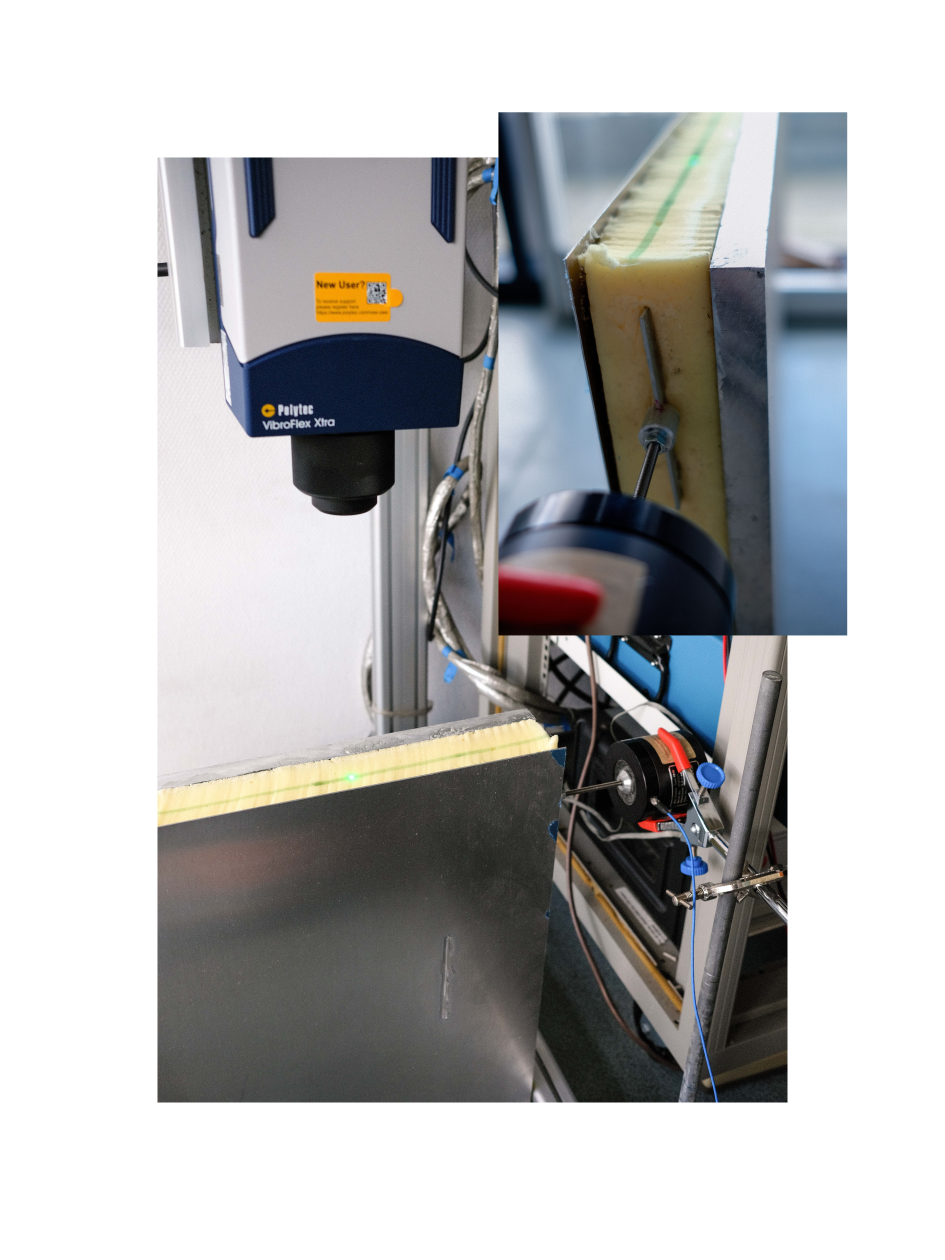
\includegraphics{chapitres/article_JAP/figures/expe_setup.pdf}
    \caption{a) Experimental set-up used for the measurement of the normal displacement field of the two-layer structure, with a close-up of the sample excitation. b) Real and c) imaginary parts of the dispersion relations recovered experimentally from the SLaTCoW method (black crosses) as calculated with the SCM (colored lines) and the bulk wavenumbers in the poroelastic material (magenta lines).}
    \label{fig:expe}
    \end{figure}

\section{Conclusion}
A spectral collocation method (SCM) is proposed to calculate dispersion relations for guided acoustic wave propagation in almost all multilayer dissipative structures \modif{Changer cette phrase ?}. The formalism is general enough to be able to consider arbitrary arrangements of (visco-) elastic, poroelastic, and (viscothermal-) fluid layers. Outgoing fluid radiation, leading to Leaky modes, can be accounted for. The fields in each layer is approximated by Chebyshev polynomials and discretized on the corresponding nodes. Interface conditions are implemented to couple layers together. The solution provides the full complex wavenumber-real frequency dispersion relation of the considered structure. In addition, the physical fields in each layer are directly evaluated since they are the eigenvectors associated with the eigenvalue problem giving the dispersion relation. The dispersion diagram calculated with the present SCM is validated against experimental results and that calculated with a root-finding method (M\"uller method) in a simple two-layer structure consisting of a rigidly backed poroelastic layer covered by a thin aluminum plate radiating in a fluid half-space. The semi-analytical approach underlying the root-finding method is taken a step further to solve for the wave amplitudes as well, providing a reference for the mode shapes calculated with the SCM.  The dispersion properties in such structures, as well as the direction of the energy density in each phase of the poroelastic layers using a decoupled expression for the Poynting vectors is analyzed. Results on energy transport velocity are also reported. 

This method paves the way of complex wavenumber-real frequency dispersion relation calculation and analysis of more complex structures, like layers with embedded periodic inclusions (elastic or resonant), i.e. metaporolastic surfaces.      

% \section*{Conflict of interest}
% The authors have no conflicts to disclose
% \section*{Author Contributions}
% \textbf{Mathieu Maréchal}
% Formal analysis (lead); 
% Investigation (equal); 
% Methodology (equal); 
% Software (lead); 
% Visualization (lead); 
% Writing – original draft (lead).
% \textbf{Alan Geslain}
% Writing – review \& editing (supporting); Investigation (equal). 
% \textbf{Jean-Philippe Groby}
% Formal analysis (equal);
% Methodology (equal);
% Supervision (equal);
% Writing – review \& editing (lead).
% \textbf{Vicent Romero-Garcìa}
% Formal analysis (supporting);
% Methodology (supporting);
% Supervision (equal);
% Writing – review \& editing (equal).
% \textbf{Olivier Dazel}
% Formal analysis (equal);
% Investigation (equal);
% Methodology (equal);
% Supervision (equal);
% Writing – review \& editing (equal).

% \section*{Data Availability Statement}
% The data that support the findings of this study are available from the corresponding author upon reasonable request. 

\section{Appendices}
\renewcommand{\thesubsection}{\thesection.\Alph{subsection}}
\subsection{Expression of the Biot elastic coefficients and effective parameters in poroelastic materials} \label{app:coefs}

The complex and frequency dependent density and bulk modulus of the fluid phase, which
accounts respectively for the viscous and thermal losses are \cite{johnson1987,champoux1991} as,
\begin{equation}
\begin{aligned}
 \rho_{\text{eq}}(\omega) &= \frac{\rho_{f} \alpha_{\infty}}{\phi}\left(1+\frac{\textrm{i}R_f \phi}{\rho_f \alpha_\infty\omega} \sqrt{1- \im  \omega  \rho_{f} \mu_f \left(\frac{ 2\alpha_{\infty}}{R_f \phi \Lambda}\right)^2 }\right),\\
K_{\text{eq}} &=\frac{\kappa P_{0}}{\phi}\left(\kappa-(\kappa-1)/\left(1+ \cfrac{\mathrm{i}R_f \phi}{\rho_f \alpha_\infty\text{Pr} \omega} \sqrt{1- \im\text{Pr} \omega \rho_{f} \mu_f\left( \frac{ 2\alpha_{\infty}}{R_f \phi \Lambda^{\prime}}\right)^2 }\right)\right)^{-1}, 
\end{aligned}
\end{equation}
where $\phi$ is the porosity, $\alpha_{\infty}$ is the tortuosity, $\Lambda$ and $\Lambda'$ are respectively the viscous and thermal characteristic lengths, $R_f$ is the flow resistivity, $\mu_f$ is the dynamic viscosity, $\kappa$ is the heat capacity ratio, $\rho_f$ the density of the saturating fluid, and $P_0$ is the ambient pressure.

The Biot elastic coefficients, $P$, $Q$, and $R$, are more commonly expressed in terms of the frame, $K_b$, effective fluid, $K_{eq}$, and shear, $N_s$, moduli when saturated by a light fluid as
\begin{equation}
P = K_b + \frac{4}{3} N_s + (1 - \phi)^2 \frac{K_{\text{eq}}}{\phi}; \quad Q = K_f(1- \phi), \quad R = \phi K_{\text{eq}},
\end{equation}
while the apparent densities are
\begin{equation}
\rho_{22}=\phi^{2} \rho_{eq}, \quad
\rho_{12}=\phi \rho_f-\rho_{22}, \quad
\rho_{11}=(1 - \phi) \rho_s-\rho_{12},
\end{equation}
 with $\rho_s$ the density of the solid phase.
The coefficients in Eq.~(\ref{eq:up_motion_equations}) are thus
\begin{equation}
    \hat A = K_b - \frac 2 3 N_s + \frac{K_{\text{eq}}}{\phi} ( \left( 1 + (1 - \phi) \right), \quad \hat \rho = \rho_1 + \phi \rho_f - 2 \phi^2\rho_{eq} - \frac{\rho_f^2}{\rho_{eq}}\quad
    \beta = \frac{\rho_f }{\rho_{eq}} - 2 \phi - 1, 
\end{equation}
where $\rho_1= \phi \rho_f + (1-\phi )\rho_s$ is 
the apparent density of the frame. Finally, the frame bulk modulus and shear modulus are linked by the Poisson ratio $\nu$ with $K_b=2N_s(1+\nu)/3(1-2\nu)$.

\subsection{Application to a single poroelastic layer surrounded by two fluid half-spaces}\label{app:fluid_coupled_poroelastic}
 
The dispersion relation of guided waves in a single layer of poroelastic material surrounded by two identical fluid half-spaces is considered (See Fig.\ref{fig:fluid_coupled_poroelastic}a). The poroelastic material properties are those considered in Section \ref{Disrel} and the layer thickness is $2h^{(1)}=104\textrm{ mm}$, i.e. twice the thickness of the poroelastic layer considered in the two-layer system.

    %\inputikz{tikz_poroelastic_appendix}
\begin{figure}
    \centering
    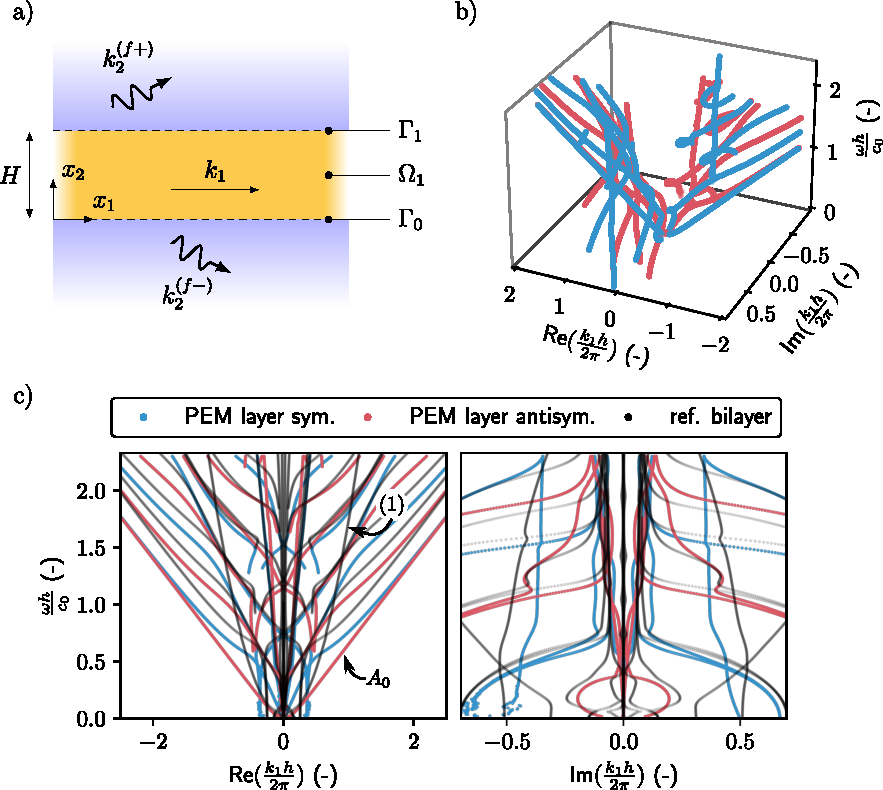
\includegraphics{chapitres/article_JAP/figures/poroelastic_appendix.pdf}
    \caption{a) Sketch of the single layer poroelastic structure geometry. b) 3D view of the complex wavenumber-real frequency dispersion relation and c) real and imaginary parts of the dispersion relation. The branches of the symmetric and antisymmetric modes are represented by blue and red curves respectively. The dispersion relation of the two-layer elatsic-poroelastic system studied in Section \ref{Section3} are reminded with black lines.}
    \label{fig:fluid_coupled_poroelastic}
\end{figure}
The discretized equations of motion is that provided in Eq.(\ref{eq:up_motion_equations_discrete}). $M^{(1)}=11$ collocation points are considered. Only the boundary conditions at the lower, i.e. $\Gamma_0$ at $x_2 = 0$, and upper, i.e. $\Gamma_1$ at $x_2 = h$, interfaces are modified. They read as \cite{debergue1999}
    \begin{equation}
        \begin{split}
            & \left(1 + \phi + \phi\frac{ \rho_{12}}{ \rho_{22}}\right)u_2^{(1)} + \frac{\phi^2}{ \rho_{22} \omega^2} \partial_2 p^{(1)} = u_2^{(0\pm)},~ 
            \quad p^{(1)}  = p^{(0\pm)},\\
            &\quad \hat \sigma_{22}^s = \left( 1 - \phi \left(1+ \cfrac{ Q} { R}\right)\right) p^{(0\pm)},~
            \quad \hat \sigma_{12}^s = 0.
        \end{split}
    \end{equation}
    
   The discretized form of these boundary conditions is
    \begin{equation}
        \nummat C_{1} = \left(
            \begin{array}{ccc|c}
                \cfrac{\phi^2}{ \rho_{22}} \numvec D_2^+ & \numvec 0 & \omega^2 \left(1 + \phi \left( 1 + \cfrac{ \rho_{12}}{ \rho_{22}}\right) \right) \numvec I^+ & \cfrac{ik_2^{(f)}}{\rho_f}  \\
                \numvec I^+ & \numvec 0 & \numvec 0 & -1 \\
                \numvec 0 & \im  k_1 (\hat P - 2 N_s) \numvec I^+ & \hat P \numvec D_2^+ & 1 - \phi \left(1+ \cfrac{ Q} { R}\right) \\
                \numvec 0 &  N_s \numvec D_2^+ & \im  k_1  N_s \numvec I^+ & 0 \\
            \end{array} \right).
            \label{eq:fluid_poro_coupling_top}
        \end{equation}
        
    %Taking a number of fields $P_1 = 3$ and a number of collocation points $M_1 = M$ for the layer makes the problem size $3M + 2$ (with 2 amplitudes terms for the radiated waves). 
    
    These matrices are then arranged in the same manner as Eq.(\ref{eq:discretized_multilayer_system}) and the wavenumbers are calculated. Fig.~\ref{fig:fluid_coupled_poroelastic}b-c depicts the results. 
    % The dispersion relation as determined with the SCM matches that calculated with the M\"uller method, thus validating the procedure. 
    
 In a similar way as Lamb modes, the different modes can be sorted in symmetric and antisymmetric modes. This is done by comparing the sign of the radiated amplitudes at each edge of the layer. Results are shown in Fig.~\ref{fig:fluid_coupled_poroelastic}b. All modes necessarily have an imaginary part, both because of the radiation condition, i.e. leakage, and because of viscothermal dissipation as can be noticed in Fig.~\ref{fig:fluid_coupled_poroelastic}c.
 
 %   It can be seen that no mode exists solely in the real plane in this configuration: from the viscothermal dissipations in the PEM, there always exists a contributing imaginary part in the wavenumber solution, and thus attenuation to the mode imaginary part of the branches of the solution are contributed from the PEM layer and not from the fluid-coupling. Small radiations are occuring at the interface, but the effect is not as strong as if it was a heavy fluid, saturating the surrounding medium and the pores of the layer, as we would have with water for example.


\subsection{Evaluation of the physical fields from the SCM solutions}
\label{app:fields}

The discrete sets of eigenvectors resulting from the SCM are the spatial Laplace transforms of some physical fields at collocation points, i.e. the locations where the discrete equations of motion (residue) are exactly satisfied. These discrete fields are interpolated into a continuous form using
\begin{equation}
    \mbf s^{(n)}(x_2) = \left[\nummat \psi_m^{-1}(\numvec \xi)  \numvec s_m^{(n)}(\numvec \xi) \right] \mbf \psi\left( \xi^{(n)} \right)
    \label{eq:reinterpolation}
\end{equation}
where the terms in brackets correspond to the coefficients $\alpha^{(n)}_m$ given in Eq.~(\ref{eq:field_to_polynomial}). The Chebyshev polynomials $\mbf \psi$ is the basis that maps from the discrete grid $\numvec \xi$ back to the physical space. 

The stress tensor components depend on the direct expressions of the fields and their first order derivative in $x_2$, denoted with a prime symbol in the following. The various fields, differentiated up to any order, can be calculated by replacing $\mbf \psi$ by its derivative in Eq.~(\ref{eq:reinterpolation}). Explicit expressions are given in the following, 
\begin{itemize}
    \item in the elastic layer, the spatial Laplace transforms of stress tensor components are computed from $\tilde{\mbf u}$, with
    \begin{equation}
    \begin{aligned}
       \tilde \sigma_{11} = (\lambda + 2\mu) &\im k_1 \tilde {\mbf u}_1 + \lambda \tilde {\mbf u}_2^\prime , \quad \tilde {\sigma}_{12} = \mu \left( \tilde {\mbf u}^\prime_1 + \im k_1 \tilde {\mbf u}_2\right), \\ &\tilde {\sigma}_{22} = \lambda \im k_1 \tilde {\mbf u}_1 + (\lambda + 2\mu) \tilde {\mbf u}_2^\prime.
    \end{aligned}
    \end{equation}
    \item in the poroelastic layer, the full solid stress tensor is expressed as $\tilde{\mbf  \sigma}_s = \mbf{\hat \sigma_s} - \phi \left( Q/R \right) \tilde{\mbf p}$, with $\mbf{\hat \sigma_s}$ the spatial Laplace transform of the \emph{in vacuo} solid stress tensor introduced in Section \ref{Section3}. The components of this full solid stress tensor are, 
    \begin{equation}
    \begin{aligned}
    \tilde {\sigma}_{s, 11} =  P \im k_1 \tilde {\mbf u}_{s,1} &+ \hat A \tilde {\mbf u}_{s,2}^{\prime} -  \phi \frac{Q}{R} \tilde {\mbf p}, \quad \tilde {\sigma}_{s, 12} = N_s \left( \tilde {\mbf u}_{s,1}^{ \prime} + \im k_1 \tilde {\mbf u}_{s,2} \right), \\ &\tilde {\sigma}_{s, 22} = \hat A \im k_1 \tilde {\mbf u}_{s,2} + P \tilde {\mbf u}_{s,2}^{ \prime} - \phi \frac{Q}{R} \tilde {\mbf p}.
    \end{aligned}
    \end{equation}
    The Laplace transform of the fluid stress tensor is calculated as 
    \begin{equation}
        \tilde {\mbf \sigma}_f = - \phi \tilde {\mbf p} \delta_{i j},
        %= Q \nabla \cdot \mbf u_f^{(1)} + R \nabla \cdot \mbf u_s^{(1)}\textcolor{red}{=....},
    \end{equation}
    and the fluid displacement components are 
    \begin{equation}
        \tilde {\mbf u}_{f, 1} = \frac{\phi}{\rho_{22}\omega^2} \im k_1 \tilde {\mbf p} - \frac{\rho_{12}}{\rho_{22}} \tilde {\mbf u}_{s, 1}, \quad
        \tilde {\mbf u}_{f, 2} = \frac{\phi}{\rho_{22}\omega^2} 
        \tilde {\mbf p}^{\prime} - \frac{\rho_{12}}{\rho_{22}} \tilde {\mbf u}_{s, 2}.
    \end{equation}
\end{itemize}
All physical fields $\theta(\mbf x)$ can finally be calculated by the inverse spatial Laplace transform with $\theta(\mbf x)=\tilde \theta(k_1,x_2)e^{\textrm{i} k_1 x_1} $. 
 
\subsection{Energy flux in the multilayer structure - Poynting theorem in a poroelastic medium}
\label{app:poynting}

Energy conservation is commonly conducted in the time domain. Let us consider a volum $\Omega$, bounded by $\partial \Omega$, with $\mbf n$ the outgoing normal vector. The energy balance or Poynting theorem in a poroelastic materials reads as \cite{biot1956,dazel2008}
\begin{equation}
        \begin{aligned} 
           - \int_{\partial \Omega} (-\mbf \sigma_s \cdot\mbf v_s^\star)\cdot  \mbf n +  (-\mbf \sigma_f \cdot \mbf v_f^\star) \cdot \mbf n ~dS
            &= \frac {1} {2} \int_\Omega \rho_1 \partial_t |\mbf v_s|^2 - \rho_{12}'\partial_t  \left(\mbf v_f - \mbf v_s \right)^2 + \rho_2 \partial_t |\mbf v_f|^2~d\Omega \\
            &+ \int_\Omega  \mbf \sigma_s : \partial_t\mbf \varepsilon_s^\star + \mbf \sigma_f :\partial_t\mbf \varepsilon_f^\star - b \left(\mbf v_s - \mbf v_f\right)^2 ~d\Omega,
        \end{aligned}
        \label{eq:poynt_energy_balance}
    \end{equation}
where $\mbf v_s=\partial_t \mbf u_s$ and $\mbf v_f=\partial_t \mbf u_f$ are the velocity fields, $\mbf \sigma_s$ and $\mbf \sigma_f$ are the stress tensors, $\mbf \varepsilon_s = 1 / 2 \left( \mbf \nabla \mbf u_s + \mbf \nabla^\transp \mbf u_s \right)$ and $\mbf \varepsilon_f = 1 / 2 \left( \mbf \nabla \mbf u_f + \mbf \nabla^\transp \mbf u_f \right)$ are the strain tensors in the solid frame and in the fluid phase respectively, and $\star$ denotes the complex conjugate. Note that a similar expression is provided in \cite{carcione1996}, where the alternative 1962 Biot formulation is used.

The left-hand side contains the energy density flux $\mbf P_s=-  \mbf \sigma_s \cdot \mbf v_s^\star$ and $\mbf P_f=-  \mbf \sigma_f \cdot \mbf v_f^\star$ in the elastic frame and fluid phase. The right-hand side contains the kinetic energy $K$ \cite{allard2009} and the internal forces $P_{\text{int}}=\partial_t W+P_{dis}$. The latter is the sum of the time derivative of the strain energy $W$ and the dissipated power $P_{dis}$ by the elastic damping and the viscous and thermal losses \cite{dazel2008}. In the frequency domain, the kinetic and strain energies read as
   \begin{equation}
        \begin{aligned}
            K = \frac 1 2 \rho_1  \partial_t |\mbf v_s|^2 - \frac 1 2 \rho_{12}' \partial_t\left(\mbf v_f - \mbf v_s \right)^2 +  \frac 1 2\rho_2 \partial_t|\mbf v_f|^2, \\
            W = \frac 1 2 \mbf{\hat \sigma_s}: \mbf \varepsilon_s^\star + \frac 1 2 R \nabla \cdot ( Q  \mbf u_s + R \mbf u_f ),
        \end{aligned}
    \end{equation}
Finally, the time average total Poynting vector is $\langle \mbf P_t \rangle=\langle \mbf P_s \rangle+\langle \mbf P_f\rangle$, with $\langle \mbf P_s \rangle=-  \textrm{Re}\left(\mbf \sigma_s \cdot \mbf v_s^\star\right)/2 $ and $\langle \mbf P_f\rangle =-  \textrm{Re}\left(\mbf \sigma_f \cdot \mbf v_f^\star \right)/2$ and the total energy density is $\langle U \rangle = \langle K \rangle+\langle W \rangle =  \text{Re}(K)/2 + \text{Re} (W)/2$. Note that a similar procedure can be followed for isotropic elastic or fluid medium \cite{royer2021}. In particular,  the elastic Umov-Poyting vector is $\langle \mbf P \rangle=\textrm{Re}\left(\mbf \sigma \cdot \mbf v^\star\right)/2$, where $\mbf \sigma$ is the stress tensor and $\mbf v$ is the velocity in the elastic medium. 

The energy transport velocity $V_e$ is evaluated from the latter expressions
\begin{equation}
    V_e = \frac{\langle \mbf P_t \rangle \cdot \mbf n}{ \langle U \rangle}.
\end{equation}
When a multi-layer configuration is considered, the latter velocity is averaged over the structure thickness $\overline{V_e} = \cfrac {\overline{P}_t} {\overline U}$, with the average Poynting vector and the average total energy defined as
\begin{equation}
    \overline{P}_t = \sum_n \frac{1}{h_n} \int_{h_{n-1}}^{h_n} \langle\mbf P_t^{(n)} \rangle\cdot \mbf e_{x_2} ~dx_2, ~~
    \overline U = \sum_n \frac{1}{h_n} \int_{h_{n-1}}^{h_n} \langle U^{(n)} \rangle  ~dx_2.
    \label{eq:mean_energy}
\end{equation}
% \printbibliography[heading=subbibnumbered]
% \end{document}